\documentclass[a4paper,10pt]{article}
\usepackage{caption}
\usepackage{cite}
\usepackage{mathtools}
\usepackage{pythonhighlight}
\usepackage{graphicx, subfigure}
\usepackage{hyperref}
\usepackage[english]{babel}
\usepackage[latin1]{inputenc}
%
\begin{document}
\captionsetup[figure]{labelfont={bf},name={Fig},labelsep=period}
%
   \title{Word2vec with Marvel Films' dialogues}

   \author{Lei Shiye}
          
   \date{2019\\ April}

   \maketitle
 
  \newpage
    
% This is a comment: in LaTeX everything that in a line comes
% after a "%" symbol is treated as comment
%\hypersetup{colorlinks=true, bookmarks, unicode}
\section*{Abstract}
% When adding * to \section, \subsection, etc... LaTeX will not assign
% a number to the section
It is always a focus that how we make machine to understand words. For instance, alligator and caiman all belong to crocodile. But how machines are aware of this? Word embedding solved this problem to some extend. It uses embedding layer to extract similarity of words and represents words by vectors.
In this report, I used a word embedding model to do word2vec project with marvel films' dialogues. And thy to find some interest relationship between these words.

\paragraph{Note:}
The source codes ralated to the report can be found on github:
\begin{verbatim} 
      https://github.com/LeavesLei/UPC-DL-lab-code/tree/master/lab_3/source_code_lab_3
\end{verbatim}

\section{Introduction}
\subsection{dataset}
I extract these movies' dialogues from Interned including:
    \begin{itemize}
      \item  Avengers series (\uppercase\expandafter{\romannumeral1}, \uppercase\expandafter{\romannumeral2}, \uppercase\expandafter{\romannumeral3})
      \item  Thor series (\uppercase\expandafter{\romannumeral1}, \uppercase\expandafter{\romannumeral2}, \uppercase\expandafter{\romannumeral3})
      \item  Iron man series (\uppercase\expandafter{\romannumeral1}, \uppercase\expandafter{\romannumeral2}, \uppercase\expandafter{\romannumeral3})
      \item  Hulk series (\uppercase\expandafter{\romannumeral1})
      \item  Captain America series (\uppercase\expandafter{\romannumeral1}, \uppercase\expandafter{\romannumeral2}, \uppercase\expandafter{\romannumeral3})
   \end{itemize}
   
There are approximately 25,000 sentences in the raw dialogue document. After being cleaning, 7,000 sentences are left.

\subsection{word embedding}
Word embedding is one of the most popular representation of document vocabulary. It is capable of capturing context of a word in a document, semantic and syntactic similarity, relation with other words, etc.

Wait a minute, I think all of beginners have this question: Why we need word embedding? I want to borrow a phrase from Hegel: What is rational is real; and what is real is rational. Generally speaking, It's easy to present word by one-hot encoder. Length of our one-hot encoded vector would be equal to the number of word in document or article. If there are just 100 words totally, one-hot encoded vector is fine. But there are usually more than 5000 words in  books. It's too flexible to use one-hot encoded vector. Besides, In one hot encoding representations, all the words are independent of each other. Is it possible that alligator is same close to crocodile and bird? Of course not. Fortunately, word embedding could overcome these difficulties.

What are word embeddings exactly? Loosely speaking, they are vector representations of a particular word. Having said this, what follows is how do we generate them? More importantly, how do they capture the context?

Word2Vec\cite{mikolov2013efficient} is one of the most popular technique to learn word embeddings using shallow neural network. It was developed by Tomas Mikolov in 2013 at Google.

\section{Methods}
\subsection{model}
Word2Vec is a method to construct such an embedding. It can be obtained using two methods (both involving Neural Networks): Skip Gram and Common Bag Of Words (CBOW)
\subsubsection{CBOW}
This method takes the context of each word as the input and tries to predict the word corresponding to the context. Consider the example: \textbf{Have a great day}. Let the input to the Neural Network be the word, great. Notice that here we are trying to predict a target word (\textbf{day}) using a single context input word great. More specifically, we use the one hot encoding of the input word and measure the output error compared to one hot encoding of the target word (\textbf{day}). In the process of predicting the target word, we learn the vector representation of the target word.

Fig \ref{Fig.single-cbow} shows the architecture of CBOW.
\begin{figure}[htpb]
\centering 
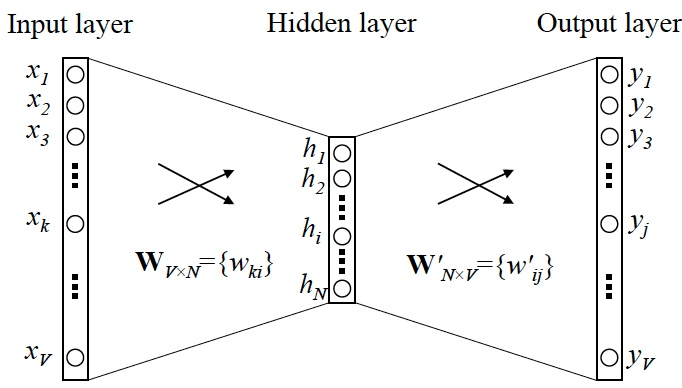
\includegraphics[width=1\textwidth]{report_image/single-cbow.jpg} 
\caption{A simple CBOW model with only one word in the context} 
\label{Fig.single-cbow} 
\end{figure}

the above model used a single context word to predict the target. We can use multiple context words to do the same, like the model in Fig \ref{Fig.multiple-cbow}

\begin{figure}[htpb]
\centering 
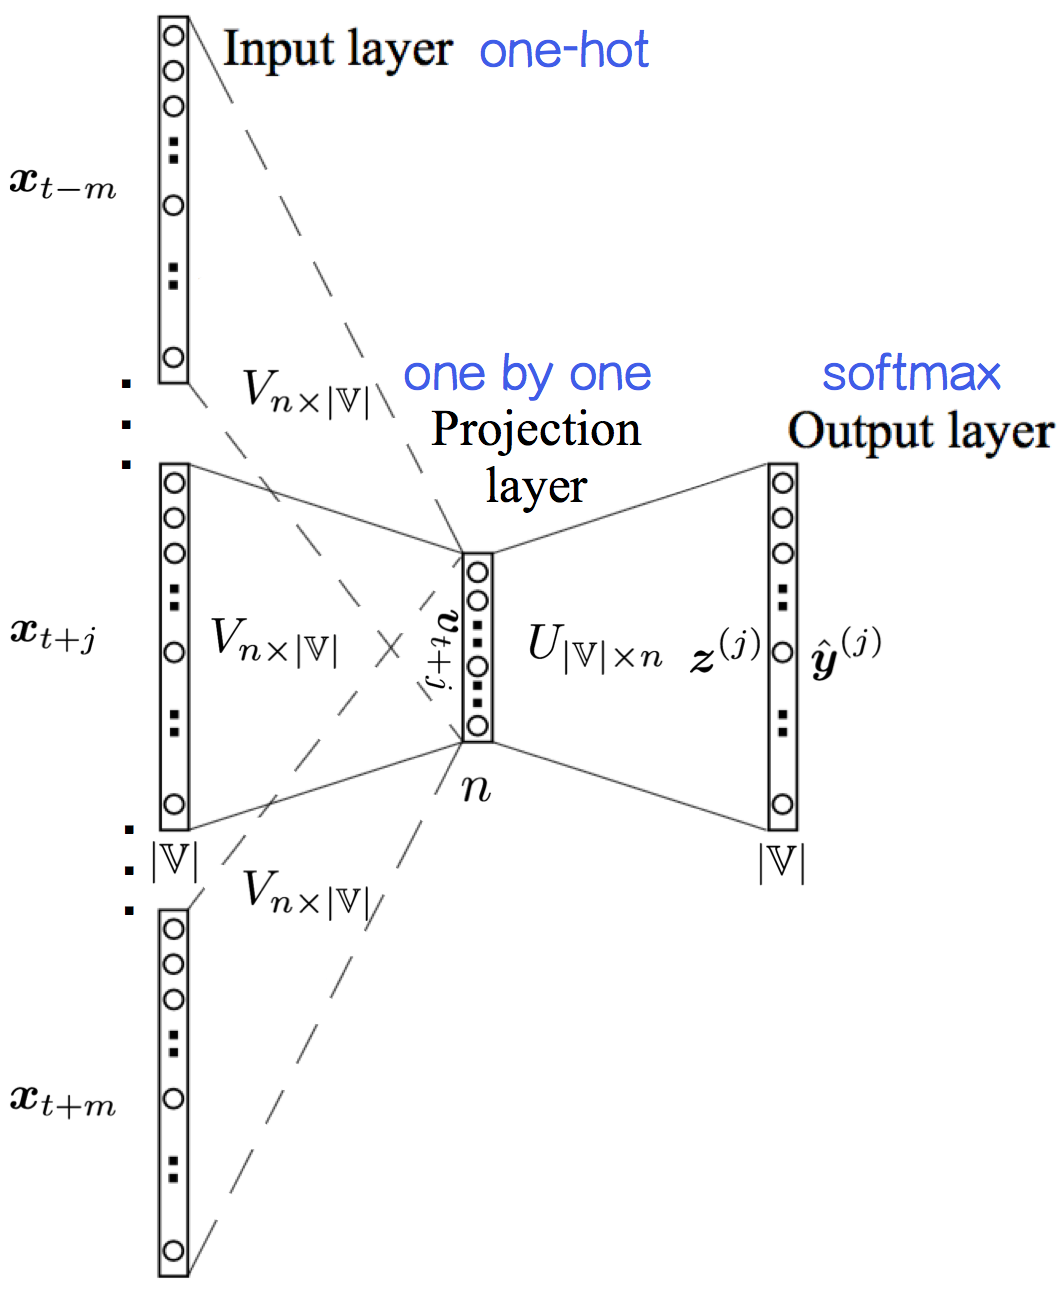
\includegraphics[width=0.5\textwidth]{report_image/mutiple-cbow.png} 
\caption{CBOW model with multiple words in the context} 
\label{Fig.multiple-cbow} 
\end{figure}

\subsubsection{Skip-Gram}
The purpose of CBOW model is to learn the probability of a word given its context. Skip-Gram is contrary to CBOW. It learns the 
probability of a context of words given a source word. the architecture is presented in Fig \ref{Fig.skip-gram}

\begin{figure}[htpb]
\centering 
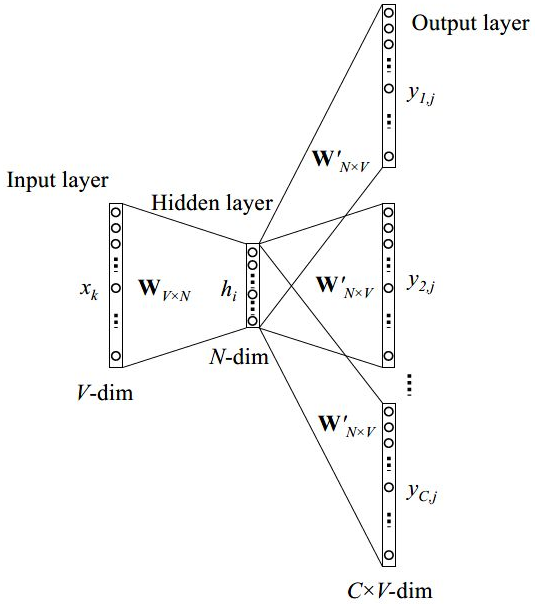
\includegraphics[width=0.5\textwidth]{report_image/skip-gram.png} 
\caption{Skip-Gram model architecture} 
\label{Fig.skip-gram} 
\end{figure}

\subsection{preprocessing}
Before putting our text into embedding model, I have done some preprocessing to achieve better results:
    \begin{itemize}
      \item  removing non-alphabetic characters.
      \item  removing stopwords. Stopwords like 'the' or 'is' are very common in text but there are pointless.
      \item  delete sentences which length less than 2. 
    \end{itemize}
   
Before preprocessing, there are about 25,000 dialogues. Only one third of them, about 7,000 sentences are retained after this part.
\subsection{Parameter setting}
I build the embedding model with $gensim$, a Python module focusing on NLP field.
There are some basic parameters in the model:
    \begin{itemize}
        \item  \textbf{$min\_count=5$}. Ignore all words with total frequency lower than 5 times.
        \item  \textbf{$window=3$}. The maximum distance between the current and predicted word within a sentence is 3.
        \item  \textbf{$size=300$}. The dimensionality of the feature vectors(word vectors) is equal to 300.
        \item  \textbf{$sg=[0,1]$}. $sg$ defines the training algorithm. By default ($sg=0$), CBOW is used. Otherwise ($sg=1$), skip-gram is employed.
        \item  \textbf{$epochs=30$}. 30 training epochs are employed in training process.
    \end{itemize}

\section{Results}
To achieve a better presentation, I want to show the basic relationship bwteen marvel films in Fig \ref{Fig.marvel}.
\begin{figure}[htpb]
\centering 
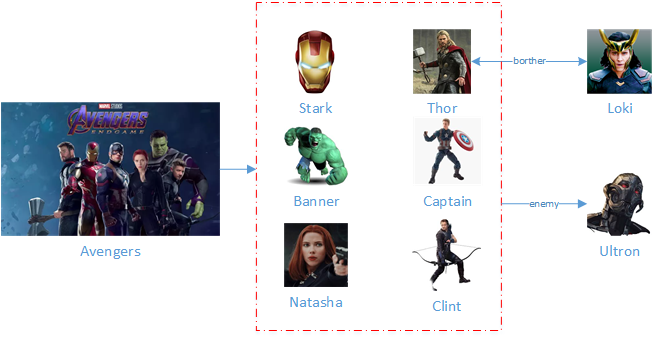
\includegraphics[width=1.0\textwidth]{report_image/marvel.png} 
\caption{Avengers relationship} 
\label{Fig.marvel} 
\end{figure}

Now we can get 10 words that are most similar to 'king':
\begin{python}
w2v_model.wv.most_similar(positive='king')
[('say', 0.4803614616394043),
 ('stark', 0.47134217619895935),
 ('need', 0.45744121074676514),
 ('loki', 0.4384043514728546),
 ('tesseract', 0.43765780329704285),
 ('kill', 0.43617480993270874),
 ('get', 0.43383070826530457),
 ('good', 0.43267160654067993),
 ('yes', 0.42987412214279175),
 ('guy', 0.4280041456222534)]
\end{python}
The result is not good. But anyway, these words except 'say' are all present power or masculinity('stark' is iron man, 'tesseract' is a treasure is marvel film).

We also can figure it out that which 2 words are more close between 3 words.
\begin{python}
w2v_model.wv.doesnt_match(['loki', 'captain', 'thor'])
'captain'
\end{python}
Loki and Thor are brothers. So Captain America should get out.
\begin{python}
w2v_model.wv.doesnt_match(['stark', 'ultron', 'banner'])
'ultron'
\end{python}
Stark and Banner both belong to Avengers. And Ultron is negative character, so he must be eliminated.
 
I use $t-SNE$\cite{maaten2008visualizing} to plot the vectors. $t-SNE$ is a non-linear dimensionality reduction algorithm that attempts to represent high-dimensional data and the underlying relationships between vectors in a lower-dimensional space.

With $t-SNE$, I've draw 'stark' and 10 of most similar words to it in Fig \ref{Fig.result-stark} though the result is not good. Let's see who are close people to our iron man.
\begin{figure}[htpb]
\centering 
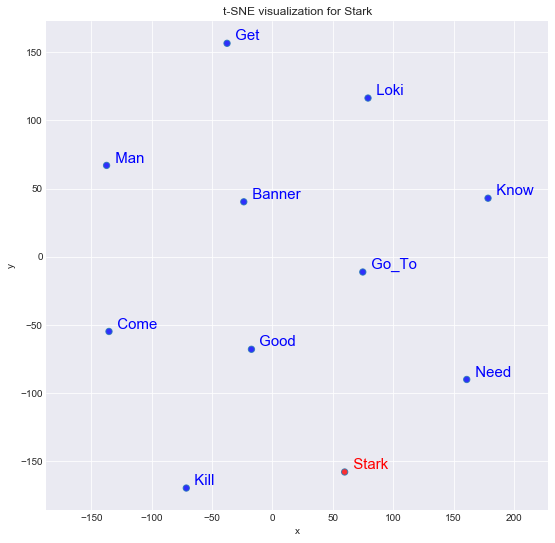
\includegraphics[width=0.6\textwidth]{report_image/result-stark.png} 
\caption{10 similar word to stark(iron man)} 
\label{Fig.result-stark} 
\end{figure}
 
All of these results are created by CBOW model. I've also used Skip-Gram model. But in the case of the result of 10 of most similar words, CBOW and Skip-Gram have a very alike performance. So I didn't present the results by using Skip-Gram model.

\section{Discussion: CBOW or Skip-Gram}
According to Mikolov, Skip-gram works well with small amount of the training data, represents well even rare words or phrases. And CBOW is faster to train than the skip-gram, slightly better accuracy for the frequent words.


But according to Google TensorFlow, CBOW smoothes over a lot of the distributional information (by treating an entire context as one observation). For the most part, this turns out to be a useful thing for smaller datasets. However, skip-gram treats each context-target pair as a new observation, and this tends to do better when we have larger datasets. 

Are the two illustrations opposite? To answer the question, we should distinguish the number of sentence and the length of sentence. 

In case of the number of sentence, predicting one word is harder than predicting a group of words, so CBOW need a larger dataset. But in case of the length of sentence, to smoothing over a lot of the distributional information, CBOW tends to prefer shorter sentences. So these two views are same explanation but just from different angles.

\section{Conclusions}
In the report I tried to do word embedding with marvel film dialogues but fail to achieve a good result. I think the main reason is my dataset. There are not only just few sentences but most of sentences are short in dataset. So the model cannot extract enough information form it. Though the eventual outcome is not successful, but I learnt a lot knowledge about word embedding form the process.

\newpage

\renewcommand\refname{Reference}
\bibliographystyle{plain}
\bibliography{ref}

\end{document}